% XCircuit output "Q_u_C.tex" for LaTeX input from Q_u_C.ps
\def\putbox#1#2#3#4{\makebox[0in][l]{\makebox[#1][l]{}\raisebox{\baselineskip}[0in][0in]{\raisebox{#2}[0in][0in]{\scalebox{#3}{#4}}}}}
\def\rightbox#1{\makebox[0in][r]{#1}}
\def\centbox#1{\makebox[0in]{#1}}
\def\topbox#1{\raisebox{-0.60\baselineskip}[0in][0in]{#1}}
\def\midbox#1{\raisebox{-0.20\baselineskip}[0in][0in]{#1}}
   \scalebox{1}{
   \normalsize
   \parbox{4.03646in}{
   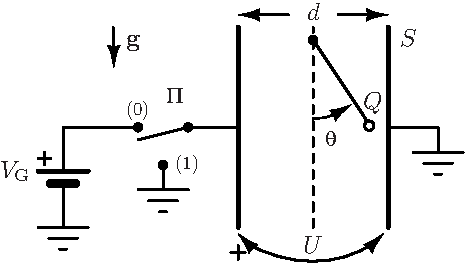
\includegraphics[scale=1]{Q_u_C}\\
   % translate x=761 y=363 scale 0.38
   \putbox{1.14in}{0.65in}{1.20}{\rightbox{\midbox{$V_\mr{G}$}}}%
   \putbox{1.85in}{1.03in}{0.90}{\centbox{(0)}}%
   \putbox{2.10in}{0.70in}{0.90}{\midbox{(1)}}%
   \putbox{3.10in}{0.86in}{1.20}{\midbox{$\uptheta$}}%
   \putbox{3.60in}{1.53in}{1.20}{\midbox{$S$}}%
   \putbox{3.02in}{1.70in}{1.20}{\centbox{\midbox{$d$}}}%
   \putbox{3.02in}{0.11in}{1.20}{\centbox{$U$}}%
   \putbox{3.35in}{1.11in}{1.20}{\midbox{$Q$}}%
   \putbox{1.77in}{1.53in}{1.20}{\midbox{$\mathbf{g}$}}%
   \putbox{2.10in}{1.11in}{1.20}{\centbox{$\Uppi$}}%
   } % close 'parbox'
   } % close 'scalebox'
   \vspace{-\baselineskip} % this is not necessary, but looks better
